\documentclass[letterpaper,12pt]{article}
\usepackage{tabularx} % extra features for tabular environment
\usepackage{amsmath}  % improve math presentation
\usepackage{graphicx} % takes care of graphic including machinery
\usepackage[margin=1in,letterpaper]{geometry} % decreases margins
%\usepackage{cite} % takes care of citations
\usepackage[final]{hyperref} % adds hyper links inside the generated pdf file
\hypersetup{
	colorlinks=true,       % false: boxed links; true: colored links
	linkcolor=black,        % color of internal links
	citecolor=blue,        % color of links to bibliography
	filecolor=magenta,     % color of file links
	urlcolor=blue,  
	pdftitle={769684}
}
\usepackage{blindtext}

\setlength\parindent{0pt}

\usepackage{flexisym}   % gives \textprime
\usepackage{amssymb}    % \mathbb{R}
\usepackage{amsmath,empheq}     % better align environment?

\usepackage{todonotes} % use \todo[inline]{text}
\renewcommand{\abstractname}{\vspace{-\baselineskip}} % drop "Abstract" from the name of the abstract
\usepackage[section]{placeins}  % force figure to appear in section

\usepackage{mathrsfs} % gives \mathscr{...} for even curlier \mathcal
\def\deleq{\overset{\Delta}{=}}


\usepackage{listings}


\usepackage[framed]{matlab-prettifier}  % use [numbered] for numbers here
\lstset{
    literate            = {-}{-}1,  % protect - in code
    style               = Matlab-editor,
    basicstyle          = \mlttfamily,
    escapechar          = ",
    mlshowsectionrules  = true,
    columns				= fullflexible, % allows copypaste
}

\usepackage{subcaption}

% Citations / bibliography
% File at ~/aalto/courses/bibliography.bib
\usepackage[backend=bibtex]{biblatex}
\addbibresource{/home/jani/aalto/courses/bibliography.bib}

%++++++++++++++++++++++++++++++++++++++++
% Commands
\newcommand{\Matlab}{\textsc{Matlab} }
\newcommand\seteq{\stackrel{\mathclap{\tiny\mbox{set}}}{=}}
%\newcommand\defeq{\stackrel{\mathclap{\normalfont\mbox{def}}}{=}}
\newcommand{\bi}{\begin{itemize}}
\newcommand{\ei}{\end{itemize}}
\newcommand{\oneitem}[2][-{}]{\bi \item[#1] #2 \ei}
\newcommand{\deq}{\triangleq}
\newcommand{\id}{\text{d}}
%++++++++++++++++++++++++++++++++++++++++

\begin{document}

\title{CHEM-E7225 Advanced Process Control \\
        Homework Report
        }

\author{Jani Arponen - 769684}
\date{\today}
\maketitle

This document contains all exercise solutions for the Advanced Process Control course. All code is publicly available at \url{https://github.com/jk-arp/apc-exercises} until the course is graded.

\section*{Exercise 01}
\textit{Consider a perfectly mixed continuous stirred tank chemical reactor (CSTR). Mass and energy balances lead to the following nonlinear dynamics}
\begin{equation} \label{eq:cstr1}
\begin{aligned}
	\frac{dC_A(t)}{dt} &= \frac{F_{\text{in}}(C_{A_{\text{in}}} - C_A(t))}{\pi r^2 h} - k_0 \exp\left(-\frac{E}{RT(t)}\right)C_A(t) \\
	\frac{dT(t)}{dt} &= \frac{F_{\text{in}}(T_{\text{in}} - T(t))}{\pi r^2 h} + \frac{-\Delta H}{\rho C_p}k_0 \exp\left(-\frac{E}{RT(t)}\right) + \frac{2U}{r\rho C_p}(T_c(t) - T(t)) \\
	\frac{dh(t)}{dt} &= \frac{F_{\text{in}} - F(t)}{\pi r^2} \\
	\mathbf{x}(t) &= \begin{bmatrix}
		C_A(t) & T(t) & h(t)
	\end{bmatrix}^T,\quad \mathbf{u}(t) = \begin{bmatrix}
		F(t) & T_c(t)
	\end{bmatrix}^T
\end{aligned}
\end{equation}

In the given source \cite{CSTR} for the exercise description, the reactor's temperature state $T(t)$ equation is slightly different (eq 1C in \cite{CSTR}) and I have used the source version going forward instead:
\begin{equation} \label{eq:cstr2}
\begin{aligned}
	\frac{dT(t)}{dt} &= \frac{F_{\text{in}}(T_{\text{in}} - T(t))}{\pi r^2 h} + \frac{-\Delta H}{\rho C_p}k_0 \exp\left(-\frac{E}{RT(t)}\right)\textcolor{red}{C_{A}(t)} + \frac{2U}{r\rho C_p}(T_c(t) - T(t)) \\
\end{aligned}
\end{equation}

\subsubsection*{Integration schemes for simulation}
The main script from the provided \texttt{dynSim.zip} was modified to use the CSTR system by writing a helper function file \texttt{CSTRfun.m}. As a first test, the system was simulated using the provided steady state values producing the graphs in Figure \ref{img:1-ss}. The \texttt{ode45} solution does not seem stable and thus an additional option to reduce the relative tolerance, shown in Figure \ref{img:1-ss-reltol}. The tank level stays constant as $\dot{h}(t) = 0$ with the given parameters and steady state values. Different constant controls were used to test the integrators and results are seen in the below graphs of Figure \ref{img:1-1}.

\begin{figure}[!htbp]
	\centering
	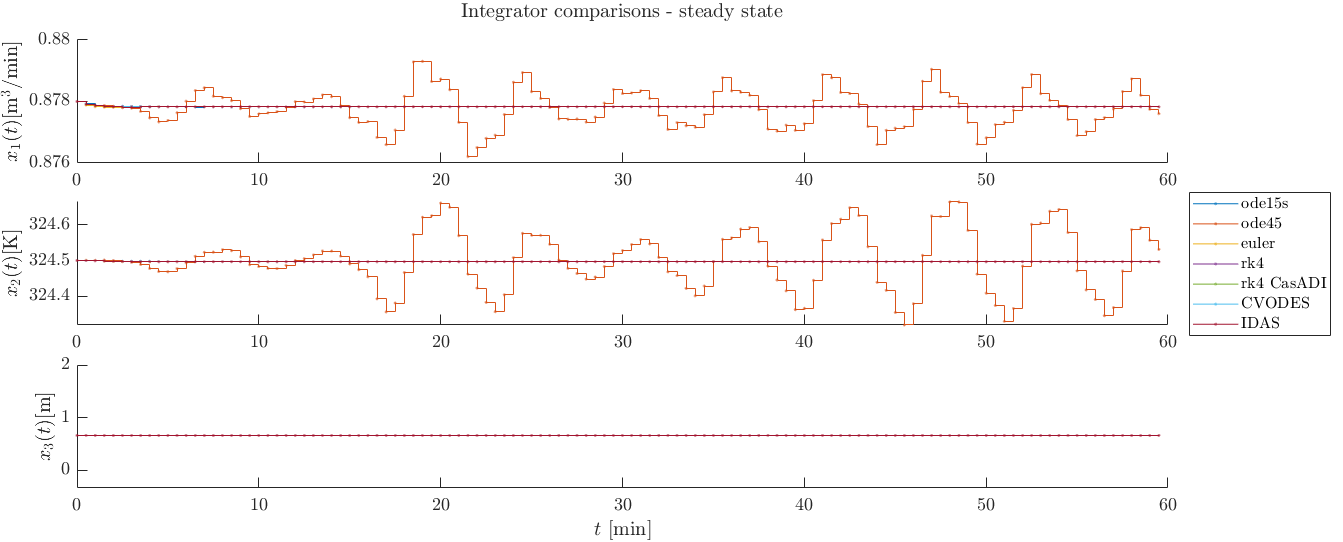
\includegraphics[width=1\textwidth]{img/1-ss.png}
	\caption{CSTR simulated at steady state control and state variable values.}
	\label{img:1-ss}
\end{figure}
\begin{figure}[!htbp]
	\centering
	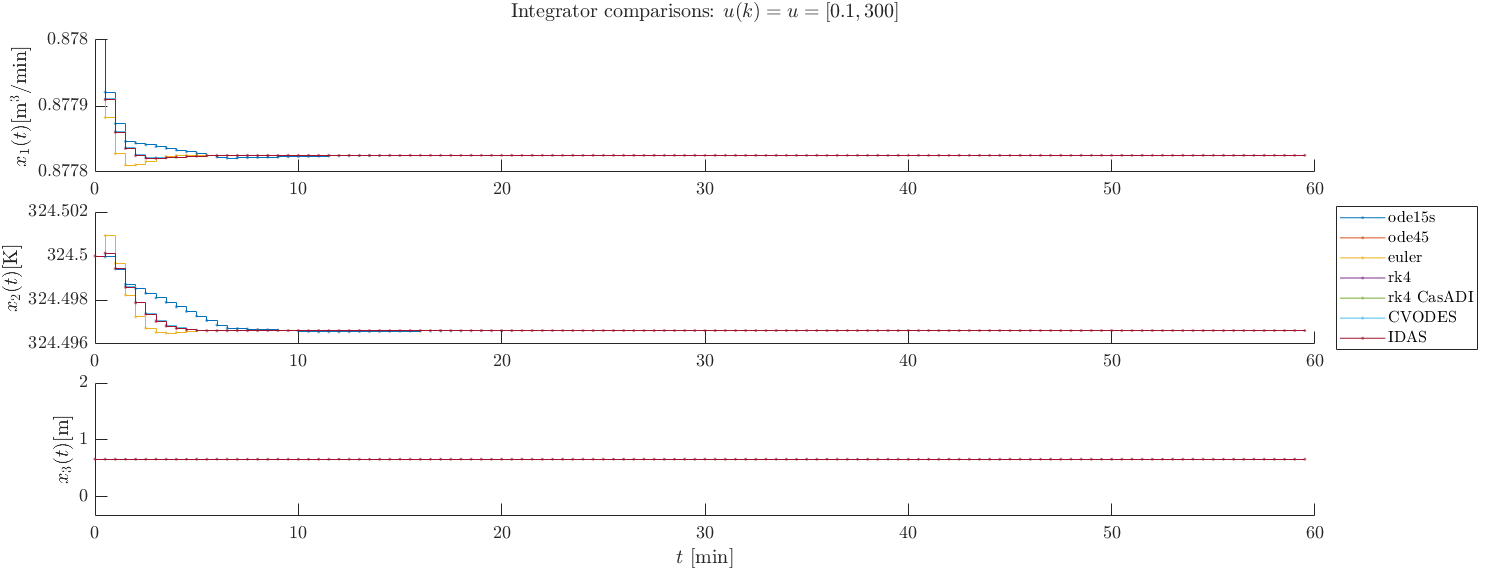
\includegraphics[width=1\textwidth]{img/1-ss-reltol.png}
	\caption{CSTR simulated at steady state control and state variable values and lower relative tolerance for the \texttt{ode45} solver.}
	\label{img:1-ss-reltol}
\end{figure}

\begin{figure}[!htbp]
\begin{subfigure}{\textwidth}
	\centering
	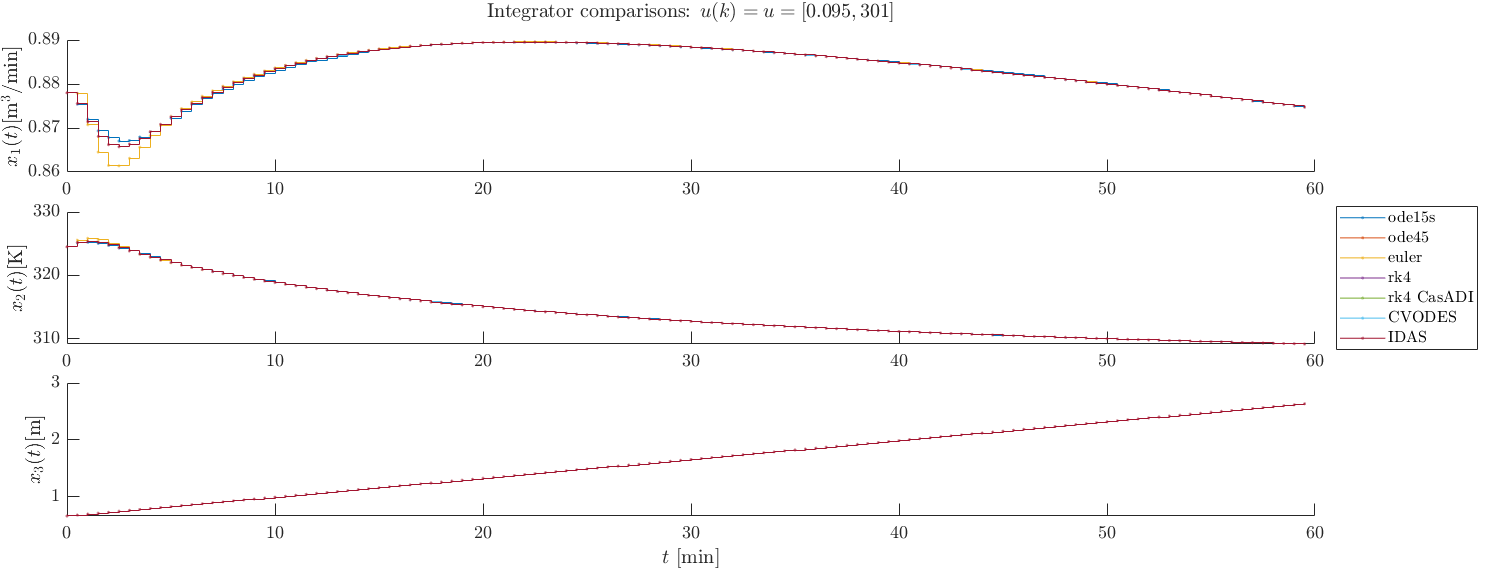
\includegraphics[width=1\textwidth]{img/1-1.png}
	\caption{}
\end{subfigure}
\begin{subfigure}{\textwidth}
	\centering
	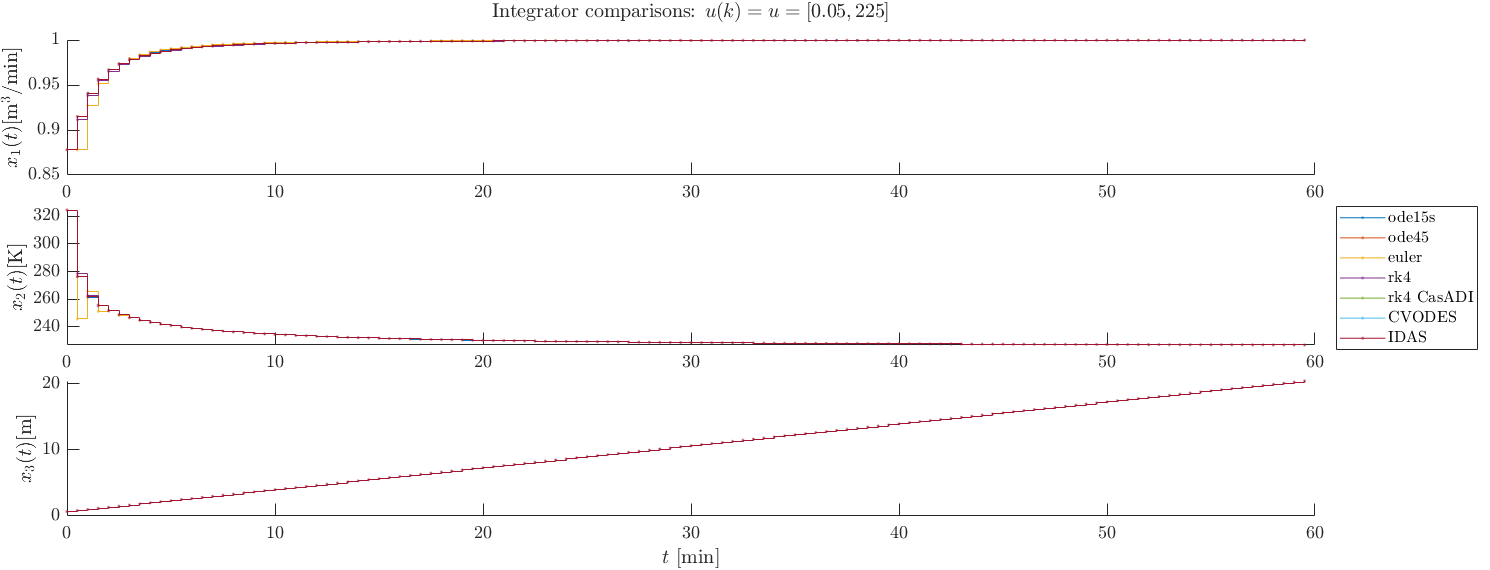
\includegraphics[width=1\textwidth]{img/1-2.png}
	\caption{}
\end{subfigure}
\begin{subfigure}{\textwidth}
	\centering
	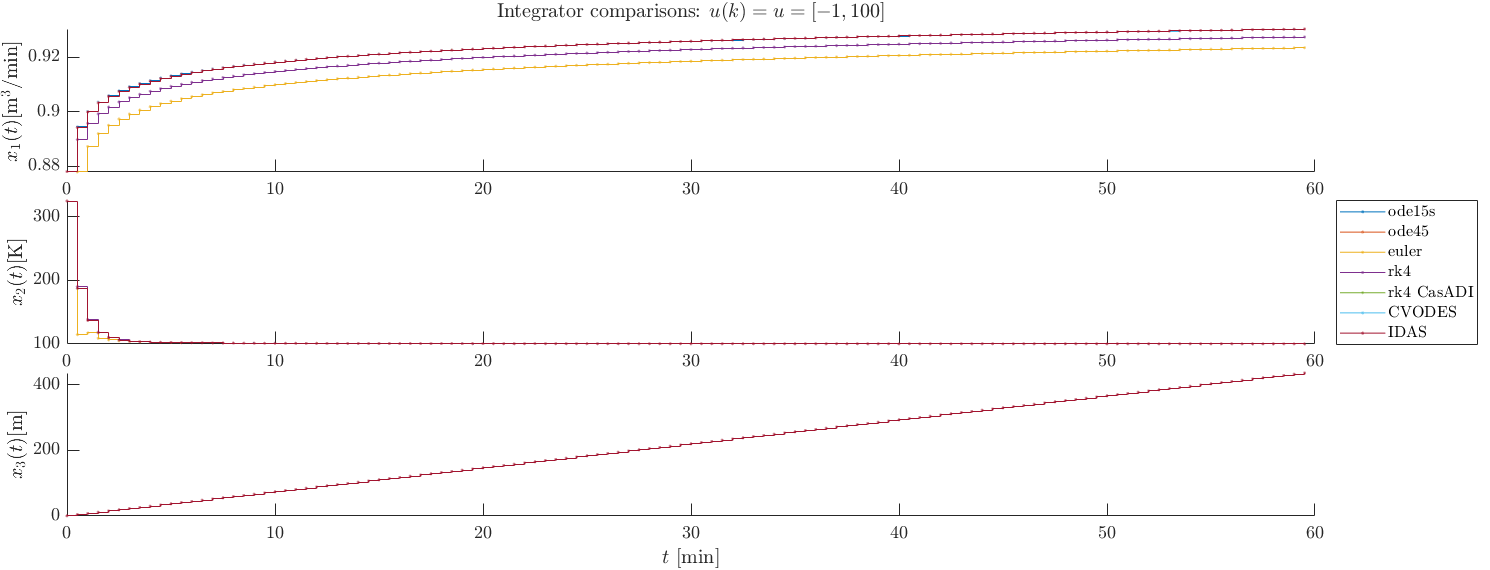
\includegraphics[width=1\textwidth]{img/1-3.png}
	\caption{}
\end{subfigure}
	\caption{CSTR simulated under different constant controls.}
	\label{img:1-1}
\end{figure}

\section*{Exercise 02}
\subsection*{Task 1}
\textit{Consider the following uni-dimensional unconstrained optimisation problem}
\begin{equation}
	\min_{x\in\mathcal{R}} \frac{x^2 - 5x + 6}{x^2 + 1}
\end{equation}

\subsubsection*{1. Plot the objective fucntion $f(x)$ and solve visually for the optimal value $x^*$}
\begin{figure}[!htbp]
	\centering
	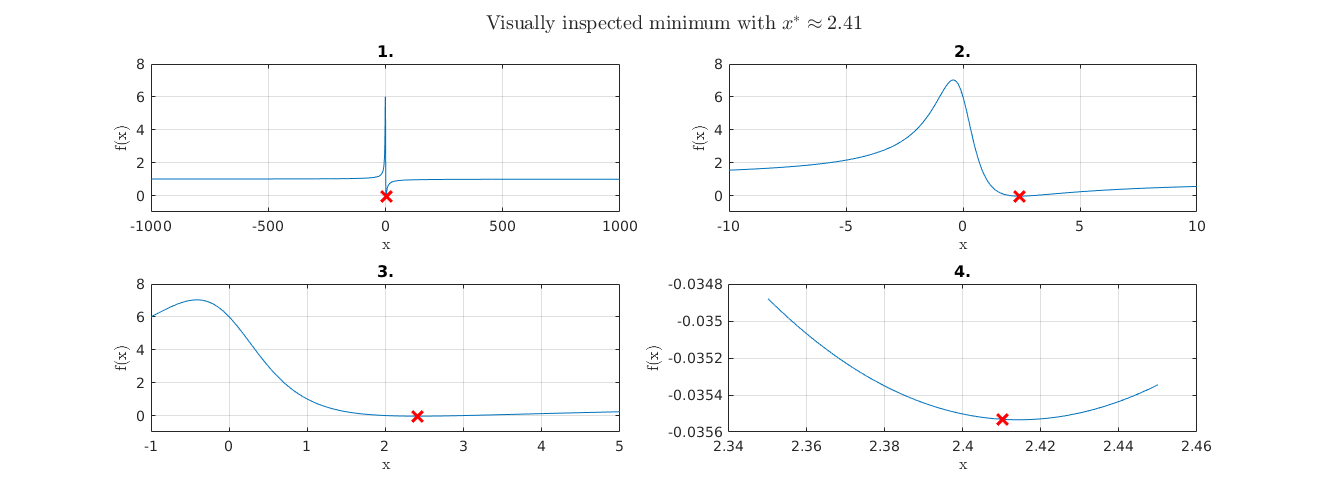
\includegraphics[width=1\textwidth]{img/2-1.png}
	\caption{The objective function plotted for different ranges of $x$ in the subfigures 1-4 to attempt a visual solution for $x^*$.}
	\label{img:2-1-visual}
\end{figure}

\subsubsection*{2. Derive on paper the gradient $\nabla f(x)$ and the Hessian $\nabla^2 f(x)$ of the objective function}
We can first obtain the gradient by the quotient rule:
\begin{equation}
\begin{aligned}
	f(x) &= \frac{x^2 - 5x + 6}{x^2 + 1} \\
	\nabla f(x) &= \frac{(2x - 5)(x^2 + 1) - (x^2 - 5x + 6)(2x)}{(x^2 + 1)^2} \\
	&= \frac{2x^3 -5x^2 + 2x -5 -2x^3 + 10x^2 - 12x}{(x^2 + 1)^2} \\
	&= \frac{5(x^2 - 2x - 1)}{(x^2 + 1)^2}
\end{aligned}
\end{equation}
and similarly for the Hessian:
\begin{equation}
\begin{aligned}
	\nabla f(x) &= \frac{5(x^2 - 2x - 1)}{(x^2 + 1)^2} \\
	\nabla^2 f(x) &= \frac{5(2x - 2)(x^2 + 1)^2 - 5(x^2 - 2x - 1)4x(x^2 + 1)}{(x^2 + 1)^4} \\
	&= \frac{10x^3 - 10x^2 + 10x - 10 - 20x^3 + 40x^2 + 20x}{(x^2 + 1)^3} \\
	&= \frac{10(-x^3 + 3x^2 + 3x - 1)}{(x^2 + 1)^3}
\end{aligned}
\end{equation}

\subsubsection*{3. Can you derive on paper the value $x^*$ such that $\nabla f(x) = 0$? If positive, comment on $\nabla^2 f(x^*)$}
We can easily solve for $x^*$ by setting the gradient to 0:
\begin{equation}
\begin{aligned}
	\nabla f(x) &= 0 \\
	\frac{5(x^2 - 2x - 1)}{(x^2 + 1)^2} &= 0 \\
	x^2 - 2x - 1 &= 0 \\
	\implies x^* = 1 \pm \sqrt{2}
\end{aligned}
\end{equation}
We now have two candidates for the minimiser and from Figure \ref{img:2-1-visual} it is clear that one of them is the minimiser and one the maximiser, since the gradient is equal to zero at both of these points. We can determine which is which by evaluating the Hessian at these points:
\begin{equation}
\begin{aligned}
	\nabla^2 f(1 + \sqrt{2}) &\approx 0.3033\\
	\nabla^2 f(1 - \sqrt{2}) &\approx -10.3033\\
\end{aligned}
\end{equation}
The first order optimality condition states that the gradient must be zero at optimal - minimal or maximal - values. The second order optimality condition can then be used to differentiate between them, by evaluating the Hessian at the optimal value(s). If the Hessian is positive semi-definite, then the optimal value is a minimiser - as is the case here with $x^* = 1 + \sqrt{2}$.

\subsubsection*{4. What would the minimiser be, had we included inequality constraints $x\in[0,4]$}
\begin{equation}
\begin{aligned}
	\min_{x\in\mathcal{R}} &\frac{x^2 - 5x + 6}{x^2 + 1} \\
	\text{subject to }& 4\geq x \geq 0
\end{aligned}
\end{equation}

The minimiser lies inside the constrained region and thus the addition of these inequality constraints would not affect the results.

\subsubsection*{5. Implement code to formulate both these problems and then solve them for the optimal values $x^*$}
Below is a snippet of the full code for this task, where \texttt{opti} is used to formulate and solve the optimization problems. 
\lstinputlisting[linerange={42-55}]{../src/exercise2_1.m}

\subsubsection*{6. Comment on the chosen solver and on the results of the optimisation.}
I decided to use \texttt{ipopt} as the solver for these problems as it was used in earlier exercises in the course and in many of the examples. Both the unconstrained and constrained solutions returned a value of approximately $2.4142$, which was expected and also equal to the minimizer $x^* = 1 + \sqrt{2}$ solved earlier.

\subsection*{Task 2}
\textit{Consider the following two-dimensional constrained optimisation problem}
\begin{equation}
\begin{aligned}
	\min_{x,y \in \mathcal{R}} &-20e^{-0.2\sqrt{0.5(x^2 + y^2)}} - e^{0.5(\cos 2\pi x + \cos 2\pi y)} + e + 20 \\
	\text{subject to } &x^2 + y^2 \leq 3
\end{aligned}
\end{equation}
\subsubsection*{1. Plot the objective function $f(x,y)$ with the feasible set and solve for the optimal value $(x^*,y^*)$}
Below, in Figure \ref{img:2-2-visual} are three different views of the objective function and the feasible set. The optimal value $(x^*,y^*) = (0,0)$ was solved visually to start with.
\begin{figure}[!htbp]
	\centering
	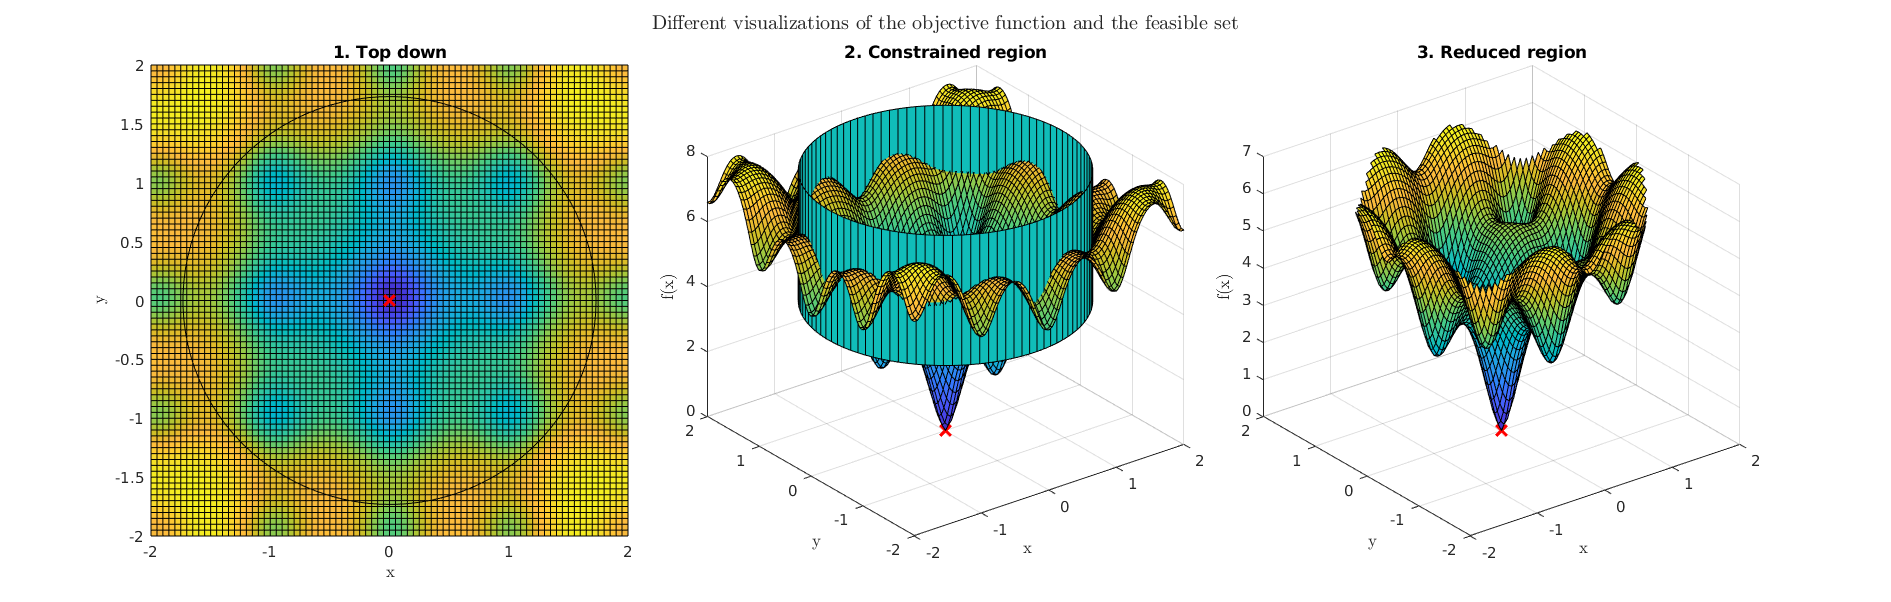
\includegraphics[width=1\textwidth]{img/2-2.png}
	\caption{The objective function plotted with different visualizations of the feasible set.}
	\label{img:2-2-visual}
\end{figure}

Taking the gradient of the objective function we get:
\begin{equation}
\begin{aligned}
	\nabla f(x,y) &= \begin{bmatrix}
		\pi e^{0.5(\cos2\pi x + \cos 2\pi y)}\sin 2 \pi x + 2x\frac{e^{-0.2\sqrt{0.5(x^2 + y^2)}}}{\sqrt{0.5(x^2 + y^2)}} \\
		\pi e^{0.5(\cos2\pi x + \cos 2\pi y)}\sin 2 \pi y + 2y\frac{e^{-0.2\sqrt{0.5(x^2 + y^2)}}}{\sqrt{0.5(x^2 + y^2)}}		
	\end{bmatrix} 
\end{aligned}
\end{equation}
We can make a noteworthy observation in the second term of the sum in both elements, namely the division by $\sqrt{0.5(x^2 + y^2)}$, which indicates that the gradient does not exist at $(0,0)$ - the visually inspected optimal point. Without loss of generality we can set $y = 0$ and take the limit
\begin{equation}
\begin{aligned}
	&\lim_{x\rightarrow 0} \pi e^{0.5(\cos2\pi x + \cos 0)}\sin 2\pi x + 2x \frac{e^{-0.2\sqrt{0.5x^2}}}{\sqrt{0.5x^2}} \\
	= &\lim_{x\rightarrow 0} 2x \frac{e^{-0.2\sqrt{0.5x^2}}}{\sqrt{0.5x^2}} \\
	\rightarrow &\lim_{x\rightarrow 0^-} (\cdots) \approx -2.8284 \\
	\rightarrow &\lim_{x\rightarrow 0^+} (\cdots) \approx 2.8284 \\
\end{aligned}
\end{equation}
and we see the discontinuity. This may raise problems in the next step of coding the optimization problem.

\subsubsection*{2. Implement code to formulate this problem and then solve it for the optimal value $(x^*,y^*)$. Show graphically and report the results when using 16 randomly chosen and different initial solutions.}
I decided to code the optimizer using the provided \texttt{simpleNewton.m} implementation of Newton's method. I modified the full step length to a fixed value of 0.2 as this seemed to produce better results at the cost of more iterations. Solutions can be seen in the below Figure \ref{img:2-2-newton} and a code snippet below that.


\begin{figure}[!htbp]
	\centering
	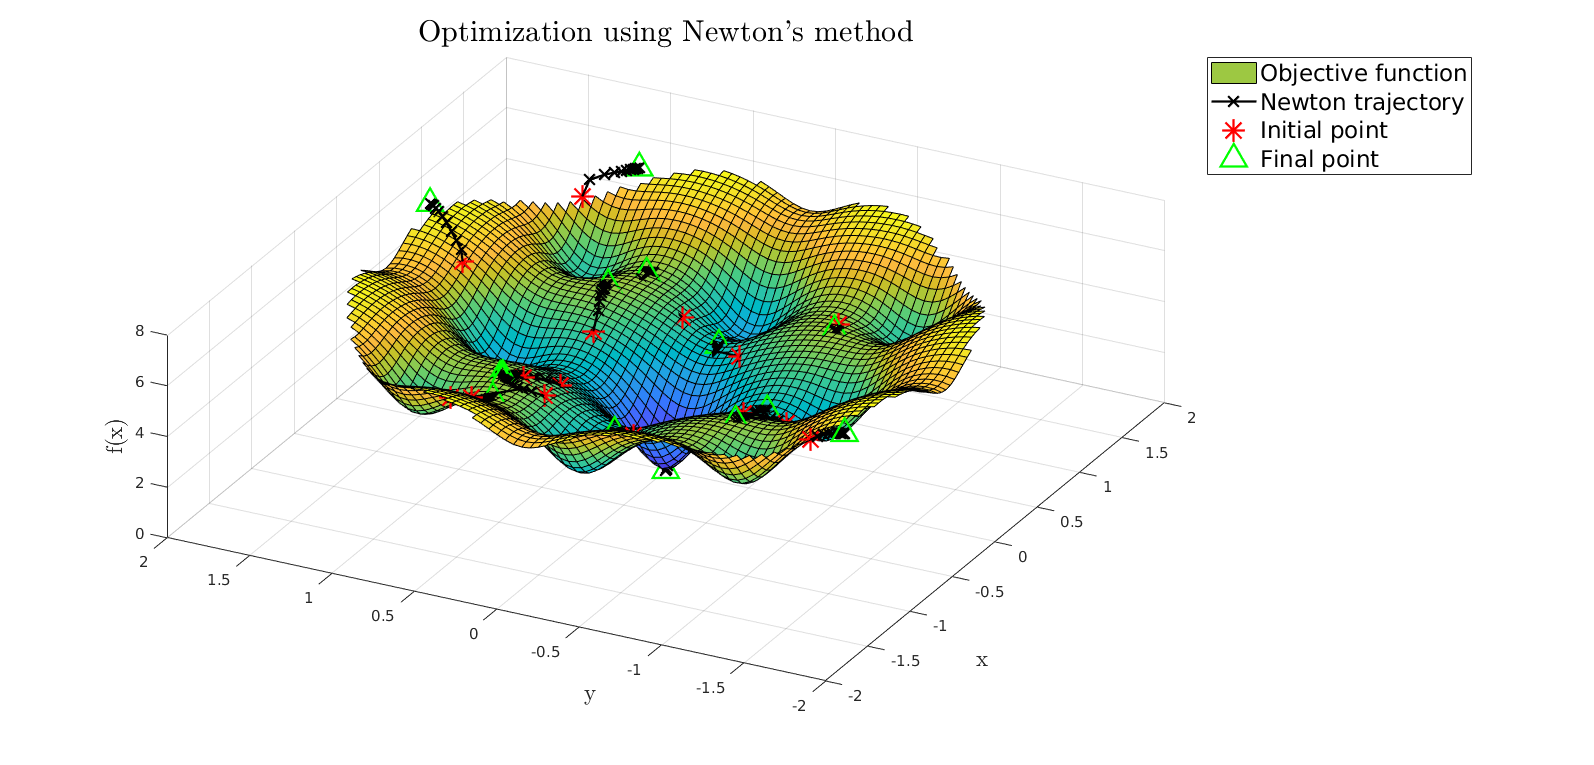
\includegraphics[width=1\textwidth]{img/2-2-newton.png}
	\caption{Optimization results using Newton's method with a fixed 0.2 step length.}
	\label{img:2-2-newton}
\end{figure}

\lstinputlisting[linerange={72-82}]{../src/exercise2_2.m}

\subsubsection*{3. Comment on the chosen solver and on the results of the optimisation.}
Newton's method performed reasonably though it needed some fine tuning for the step size and iteration count. From Figure \ref{img:2-2-newton} it is obvious that most of the solutions do not converge to the true optimal value, but rather get stuck in either saddle points or local minima and a "lucky" initial guess is needed for a global optimum. This is expected of Newton's method. An attempt was made for implementing the optimization with \texttt{ipopt} instead, but that did not seem to converge either (even with ludicrous iteration count).

\subsection*{Task 3}
\textit{Consider the constrained optimisation of the $N$-dimensional Rosenbrock function}
\begin{equation}
\begin{aligned}
	\min_{x\in\mathcal{R}^{N+1}} &\sum_{n=1}^N\left(100(x_{n+1} - x_n^2)^2 + (1 - x_n)^2\right) \\
	\text{subject to } &\sum_{n=1}^{N+1}(x_n - 1)^2 \leq 2
\end{aligned}
\end{equation}

\subsubsection*{1. Implement code to formulate this problem for $N = 8$, then solve it from different initial solutions}
I decided to implement this problem using \texttt{ipopt} and \texttt{opti}. Evaluating the optimizer at different initial solutions was done by polling $K$ points from the $N + 1$ dimensional hypersphere defined by the inequality constraint function \cite{randsphere}. Code snippet below.

\lstinputlisting[linerange={6-33}]{../src/exercise2_3.m}


\subsubsection*{2. Solve for the optimal value $x^*$ and comment on the chosen solver and on the results of the optimisation}
All of the randomly chosen initial points resulted in an optimal point $\mathbf{x}^* = \begin{bmatrix}1& 1 & \cdots& 1\end{bmatrix}^T$, which is the well known global minima of this n-dimensional extension of the Rosenbrock system \cite{rosenbrockwiki}. 

\section*{Exercise 03}
\textit{Consider the following optimal control problem for the CSTR system from Exercise 01 (eq \ref{eq:cstr1} and \ref{eq:cstr2}), where the control variable boundaries are expressed as element wise inequalities}
\begin{equation}
\begin{alignedat}{2}
	\min_{\substack{x(0\rightsquigarrow t_f) \\ u(0\rightsquigarrow t_f) }} & E(\mathbf{x}(t_f)) + 
		\int_0^{t_f} L(\mathbf{x}(t),\mathbf{u}(t))dt \\
	\text{subject to } & \dot{\mathbf{x}}(t) = \mathbf{f}(\mathbf{x}(t),\mathbf{u}(t),\mathbf{d}(t) | \theta_{\mathbf{x}}),  && t \in [0, T] \\
	& \mathbf{u}_{\text{max}} \leq \mathbf{u}(t) \leq \mathbf{u}_{\text{min}},  &&t \in [0,T] \\
	& \mathbf{x}(0) = \mathbf{x}_0  &&(t = 0)
\end{alignedat}
\end{equation}
\textit{With terminal stage - and running costs}
\begin{equation}
\begin{aligned}
	E(\mathbf{x}(t)) &= \frac{1}{2}\left( (\mathbf{x}(T) - \mathbf{x}_{\text{ref}}) ^T \mathbf{Q}_{t_f} (\mathbf{x}(T) - \mathbf{x}_{\text{ref}}) \right) \\
	L(\mathbf{x}(t),\mathbf{u}(t)) &= \frac{1}{2}\left[ (\mathbf{x}(t) - \mathbf{x}_{\text{ref}}) ^T \mathbf{Q} (\mathbf{x}(t) - \mathbf{x}_{\text{ref}}) + (\mathbf{u}(t) - \mathbf{u}_{\text{ref}}) ^T \mathbf{R} (\mathbf{u}(t) - \mathbf{u}_{\text{ref}}) \right] \\
	& \mathbf{Q}_{t_f}, \mathbf{Q} \succeq 0, \quad \mathbf{R} \succ 0
\end{aligned}
\end{equation}
\textit{The state equations and parameters are the same as used in Exercise 01. The reference state and control values are the steady state ones from Exercise 01 and the initial state is:}
\begin{equation}
\begin{aligned}
	\mathbf{x}_0 &= \begin{bmatrix}
		0.9 & 0 & 0 \\ 0 & 1.1 & 0 \\ 0 & 0 & 1.0
	\end{bmatrix} \mathbf{x}_{\text{ref}}
\end{aligned}
\end{equation}
\textit{The upper- and lower-bounds of control are:}
\begin{equation}
\begin{aligned}
	\mathbf{u}_{\text{min}} &= 0.85 \mathbf{u}_{\text{ref}} \\
	\mathbf{u}_{\text{max}} &= 1.15 \mathbf{u}_{\text{ref}} 
\end{aligned}
\end{equation}

\subsubsection*{Discrete-time optimal control formulation}
Discretizing the system is simple when the control is assumed constant over the discretization interval:
\begin{equation}
\begin{alignedat}{2}
	\dot{\mathbf{x}}(t) &= \mathbf{f}(\mathbf{x}(t),\mathbf{u}(t)|\theta_{\mathbf{x}})  && t \in [0,T]\\ 
	\mathbf{x}(t + \Delta t) &= \mathbf{x}(t) + \int_{t}^{t + \Delta t}\mathbf{f}(\mathbf{x}(\tau),\mathbf{u}(\tau)|\theta_{\mathbf{x}})d\tau && \\
	&\approx \mathbf{x}(t) + \int_{t}^{t + \Delta t}\mathbf{f}(\mathbf{x}(\tau),\mathbf{u}_{k}(\tau)|\theta_{\mathbf{x}})d\tau && \\ \mathbf{u}_{k}(\tau) &= \mathbf{u}(t = k\Delta t)\ \forall\ \tau \in [k\Delta t, (k + 1)\Delta t) &&	\\
	\mathbf{x}(t + \Delta t) &\approx \mathbf{x}(t) + \mathbf{f}(\mathbf{x}(t),\mathbf{u}_k(t)|\theta_{\mathbf{x}})\Delta t && \\
	k\Delta t &\deleq t, \quad (k + 1)\Delta t \deleq t + \Delta t, \quad K\Delta t \deleq T && \\
	\rightarrow \mathbf{x}_{k + 1} &\approx \mathbf{x}_k + \mathbf{f}(\mathbf{x}_k, \mathbf{u}_k| \theta_{\mathbf{x}})\Delta t &&	 k \in [0, 1, \cdots K]
\end{alignedat}
\end{equation}

The code for the sequential and simultaneous solutions was based on the code provided during the course in \texttt{toyOCP.zip} and further edited to fit the problem description. A final time of $t_f = 10$ minutes and a total of $K = 250$ steps was chosen through experimentation leading to a timestep of $\Delta t \approx 10ms$. A smaller step count may have sufficed, but numerical issues with the sequential approach seemed to be easier to deal with using a smaller timestep.


\subsubsection*{Sequential solution}
Eliminating the state variables from the discretized system is done by writing the states as a sequence of controls, i.e.
\begin{equation}
\begin{aligned}
	\mathbf{x}_{1} &= \mathbf{x}_0 + \mathbf{f}(\mathbf{x}_0, \mathbf{u}_1|\theta_{\mathbf{x}})\Delta t \\
	\mathbf{x}_{2} &= \mathbf{f}(\mathbf{x}_0, \mathbf{u}_1|\theta_{\mathbf{x}})\Delta  + \mathbf{f}(\mathbf{f}(\mathbf{x}_0, \mathbf{u}_1)|\theta_{\mathbf{x}}),\mathbf{u}_2|\theta_{\mathbf{x}}) \\
	&\ \ \vdots \\
	\mathbf{x}_{k + 1} &= \mathbf{f}(\mathbf{f}(\cdots \mathbf{f}(\mathbf{x}_0,\mathbf{u}_1|\theta_{\mathbf{x}}),\cdots)\mathbf{u}_k|\theta_{\mathbf{x}})
\end{aligned}
\end{equation}

The simulation results for the sequential solution can be seen in Figure \ref{img:3-seq}. Through multiple different parameters, the control for the sequential solution always seemed to fail on numerical issues for when $x_3$ gets a value close to 0 thus blowing up the derivatives due to the volume calculation for the first two states. The regulator parameters used for the included graphs were:
\begin{equation}
\begin{aligned}
	\mathbf{Q}_{t_f} &= 10^6\mathbf{Q},\ \mathbf{Q} = \mathbf{I}^{(3\times3)},\ \mathbf{R} = \mathbf{I}^{(2\times2)}
\end{aligned}
\end{equation}

\begin{figure}[!htbp]
	\centering
	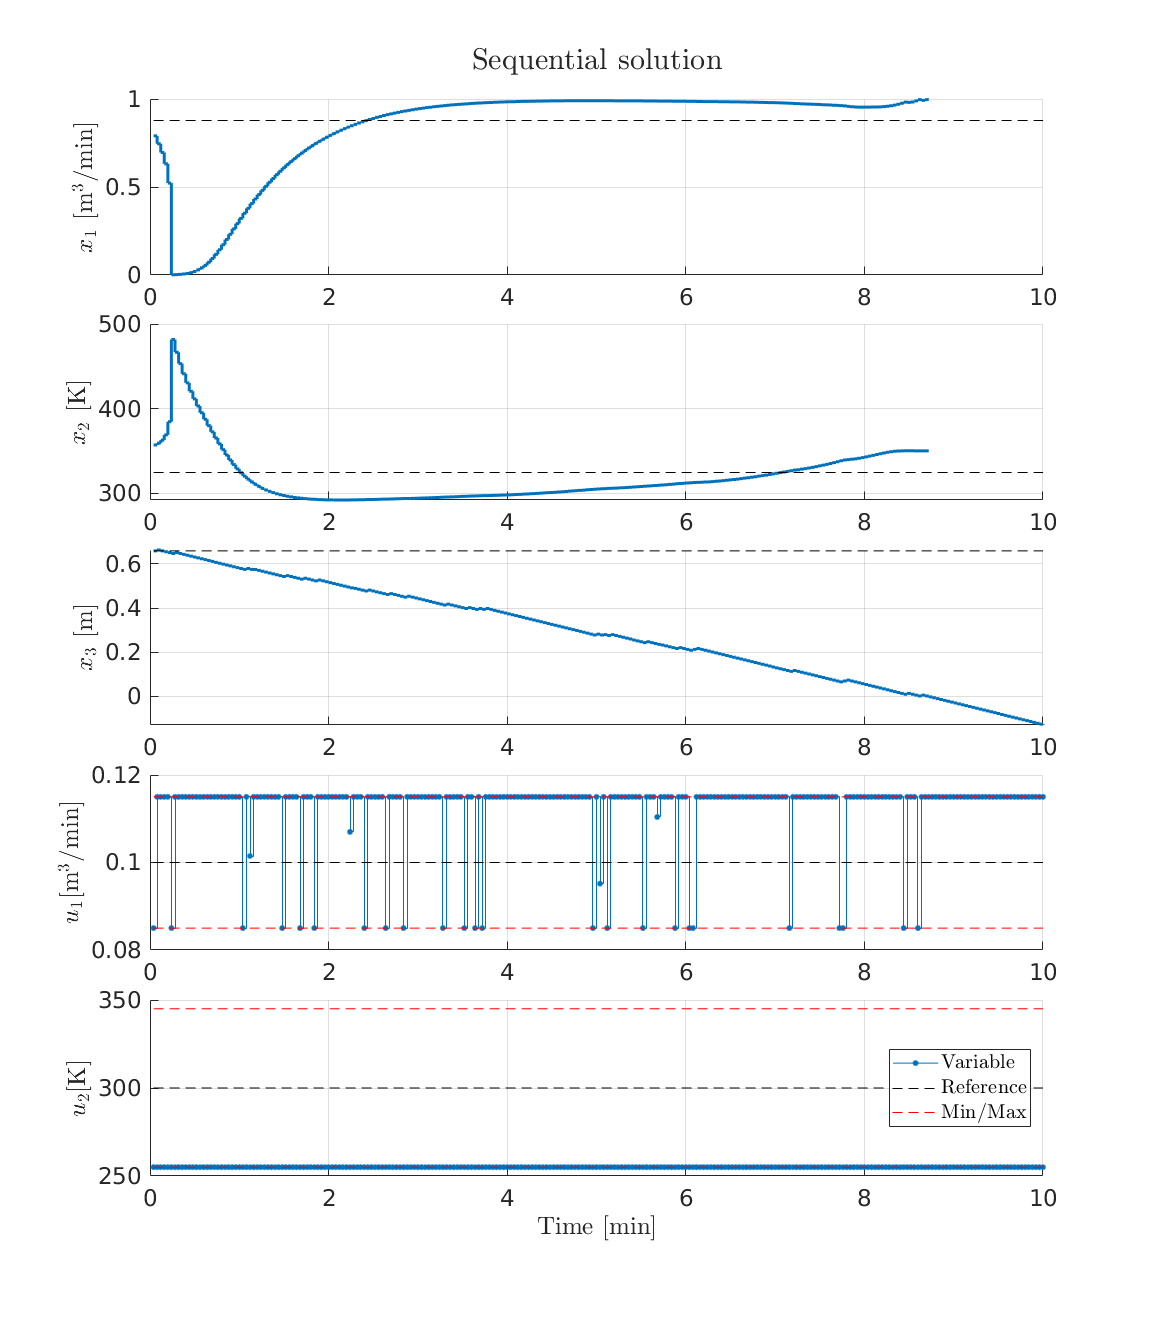
\includegraphics[width=1\textwidth]{img/3-seq.png}
	\caption{Solution to the optimal control problem using the sequential approach. Each state and control variable plotted separately with their respective reference and boundary values.}
	\label{img:3-seq}
\end{figure}


\subsubsection*{Simultaneous solution}
The simulation results for the simultaneous solution can be seen in Figure \ref*{img:3-sim}. The simultaneous solution required adding a lower limit on the states such that the none of them could be zero or negative in addition to the bounds on the control variables. The regulator parameters used for the included graphs were:

\begin{equation}
\begin{aligned}
	\mathbf{Q} _{t_f} &= 10^6 \mathbf{Q},\ \mathbf{Q} = \begin{bmatrix}
		100 & 0 & 0 \\ 0 & 10 & 0 \\ 0 & 0 & 0
	\end{bmatrix},\ \mathbf{R} = \begin{bmatrix}
		0.1 & 0 \\ 0 & 0.1
	\end{bmatrix}
\end{aligned}
\end{equation}

\begin{figure}[!htbp]
	\centering
	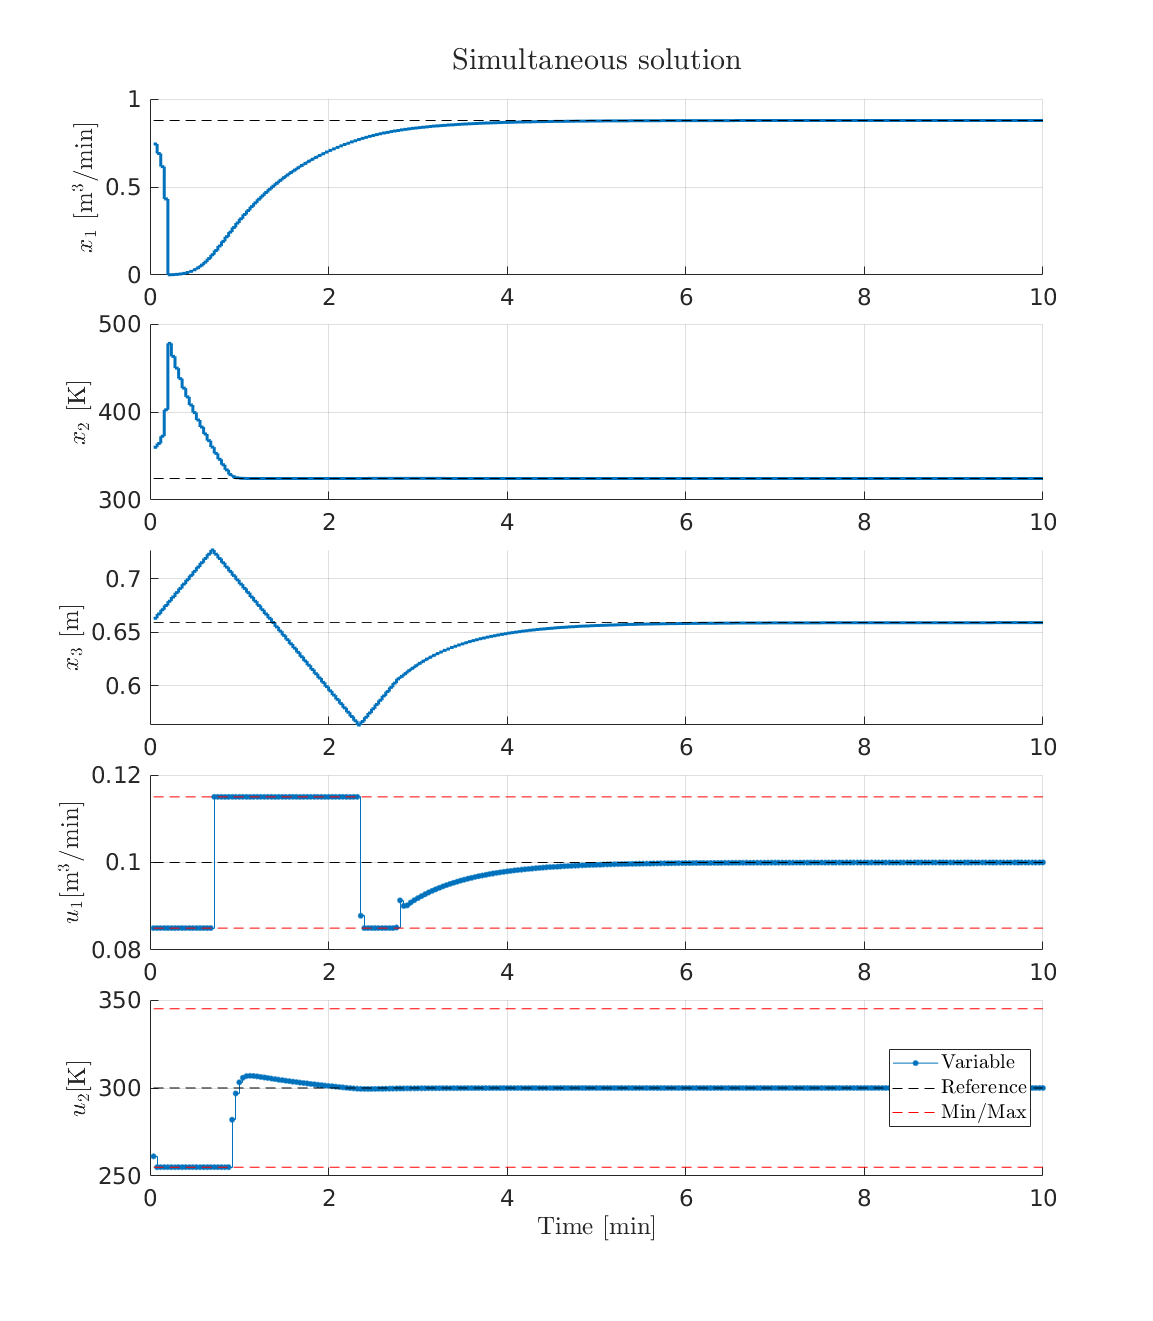
\includegraphics[width=1\textwidth]{img/3-sim.png}
	\caption{Solution to the optimal control problem using the simultaneous approach. Each state and control variable plotted separately with their respective reference and boundary values.}
	\label{img:3-sim}
\end{figure}


% \begin{figure}[!htbp]
%     \centering
%     \includegraphics[width=0.7\textwidth]{hw2-desc-2.png}
%     \caption{Given problem description. Assuming the $G_t$ next to the receiver is $G_r$.}
%     \label{img:prob2}
% \end{figure}

\printbibliography
\end{document}
